\chapter{SuperCollider}

\section{¿Qué es SuperCollider?}

SuperCollider es un lenguaje de programación general orientado a objetos. Esto significa que usando texto y expresiones determinadas, podemos realizar cualquier tarea computacional usando un paradigma de jerarquias y herencia de clases. Su objetivo principal es sintetizar audio en tiempo real y componer sonidos y obras musicales mediante algoritmos. 

Dentro del contexto de software para síntesis de audio, es uno de los más versátiles y poderosos ambientes de programación gracias a su sintaxis compacta y a la inmensidad de aplicaciones y extensiones generadas por sus usuarios. SuperCollider es software de código libre y es absolutamente gratuito. Fue originalmente creado por James McCartney y esta constantemente evolucionando gracias a su muy activa comunidad. 

Es difícil explicar lo que SuperCollider es capaz de hacer precisamente por la inmensidad de opciones que ofrece. Algunos ejemplos de aplicaciones comunes:

\begin{itemize}
\item Síntesis de audio
\item Composiciones automáticas
\item Creación de instrumentos digitales
\item Live coding
\item Creación de música generativa
\item Creación de instalaciones sonoras
\item Interacción con interfaces y sensores
\item Desarrollo de software para aplicaciones científicas
\item Musíca en red
\end{itemize}

Sin embargo, podemos realizar proyectos menos comunes y más atrevidos. Por dar un ejemplo bizarro: digamos que queremos sonificar todos los tweets de una cuenta de Twitter en base a ciertas reglas propias y queremos que otras computadoras alrededor del mundo reconozcan mensajes que les digan cuando tocar ciertos sonidos en base a estos tweets. Mientras hacemos esto, queremos enviar datos a diez microcontroladores ubicados alrededor del mundo, que reaccionan de acuerdo al análisis de la señal del mercado de acciones de Google durante los últimos diez años. Cada uno de estos motores toca una campana en diferentes ciudades del mundo, sincronizadas mediante nuestra laptop en casa... ¿cómo haríamos todo esto con software estándar? Pues bien, para esto podemos usar SuperCollider.

Como ves, las aplicaciones son difíciles de definir y engloban una gran cantidad de posibilidades. A modo de ejemplo, puedes ir al link: \href{https://soundcloud.com/darien-brito/debris2-volatility-stereo-version}{\textbf{\textit{Debris[2] //volatility}}} para escuchar una pieza de música electrónica que compuse en el año 2016, cuyos sonidos fueron realizados íntegramente en SuperCollider, usando herramientas propias que escribí. Puedes también accederla en el siguiente link:

\begin{verbatim}
http://darienbrito.com/works/debris2-volatility/
\end{verbatim}

\section{Arquitectura}

Va mas allá de esta introducción el explicar en detalle cuál es la arquitectura del software en sí. Aprender eso será necesario cuando domines los conceptos básicos y comiences a desarrollar tus propias extensiones y herramientas. 

Por ahora basta con saber que SuperCollider consta de tres programas: 

\begin{enumerate}
	\item El intérprete (o cliente). Es la parte que se encarga de traducir las instrucciones que escribimos en nuestros programas de modo que el servidor las entienda.
	\item El servidor. Es la parte que se encarga de producir sonidos y valores.
	\item La interface. Es la parte en donde escribimos código, accedemos a los archivos de ayuda y supervisamos la consola\footnote{La consola es un monitor que nos muestra mensajes y notificaciones cuando ejecutamos programas. Lo usamos para controlar que nuestro código funciona bien.}. 
\end{enumerate}

Estos tres programas funcionan en sincronía cada vez que usas SuperCollider y pueden ser controlados independientemente desde la interface.

\section{Interface}

La interface de SuperCollider nos presenta tres áreas:

\begin{enumerate}
	\item El espacio de trabajo, en donde escribimos código.
	\item La ventana de ayuda, en donde encontramos documentación.
	\item La consola, en donde monitoreamos nuestros programas. 
\end{enumerate}

\begin{figure}[h]
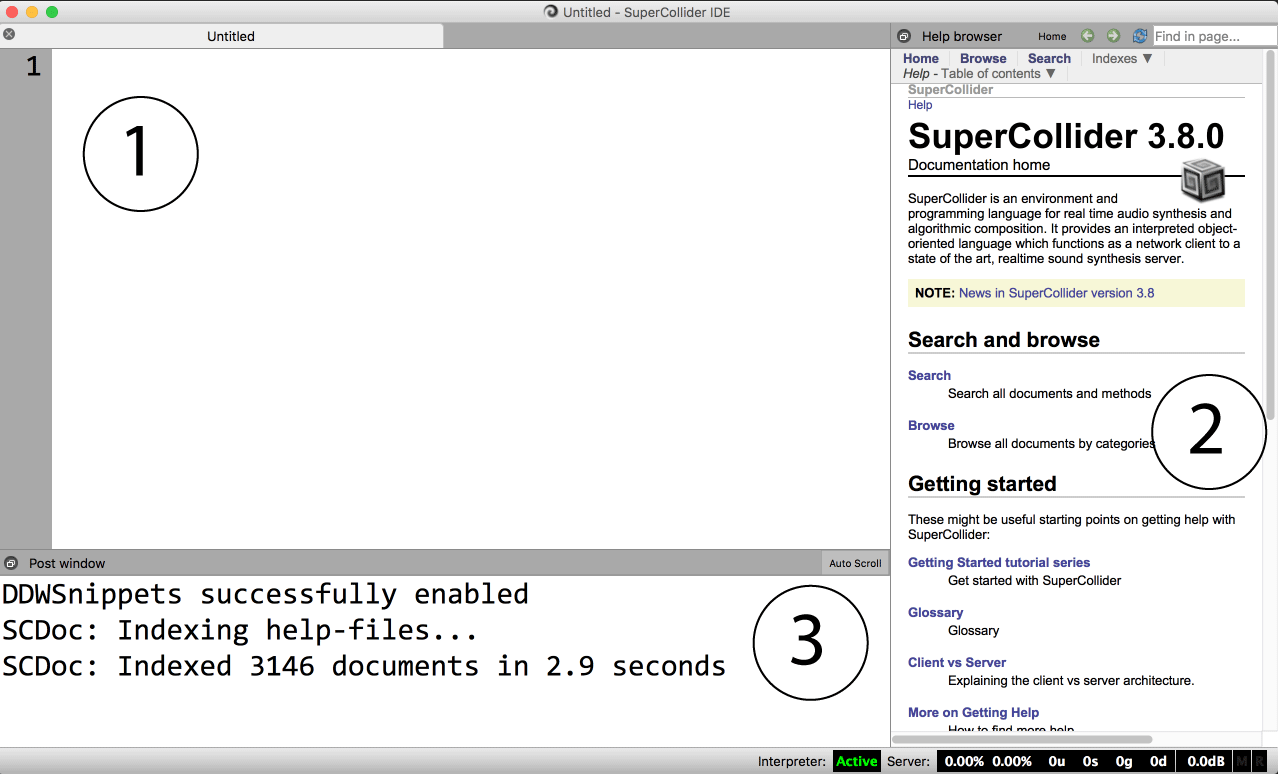
\includegraphics[scale=0.18]{interface1}
\centering
\caption{La interface}
\label{fig:áreas}
\end{figure}

Podemos configurar el modo en el que queremos ordenar esta interface haciendo click en el menú de cada ventana:

\begin{figure}[h]
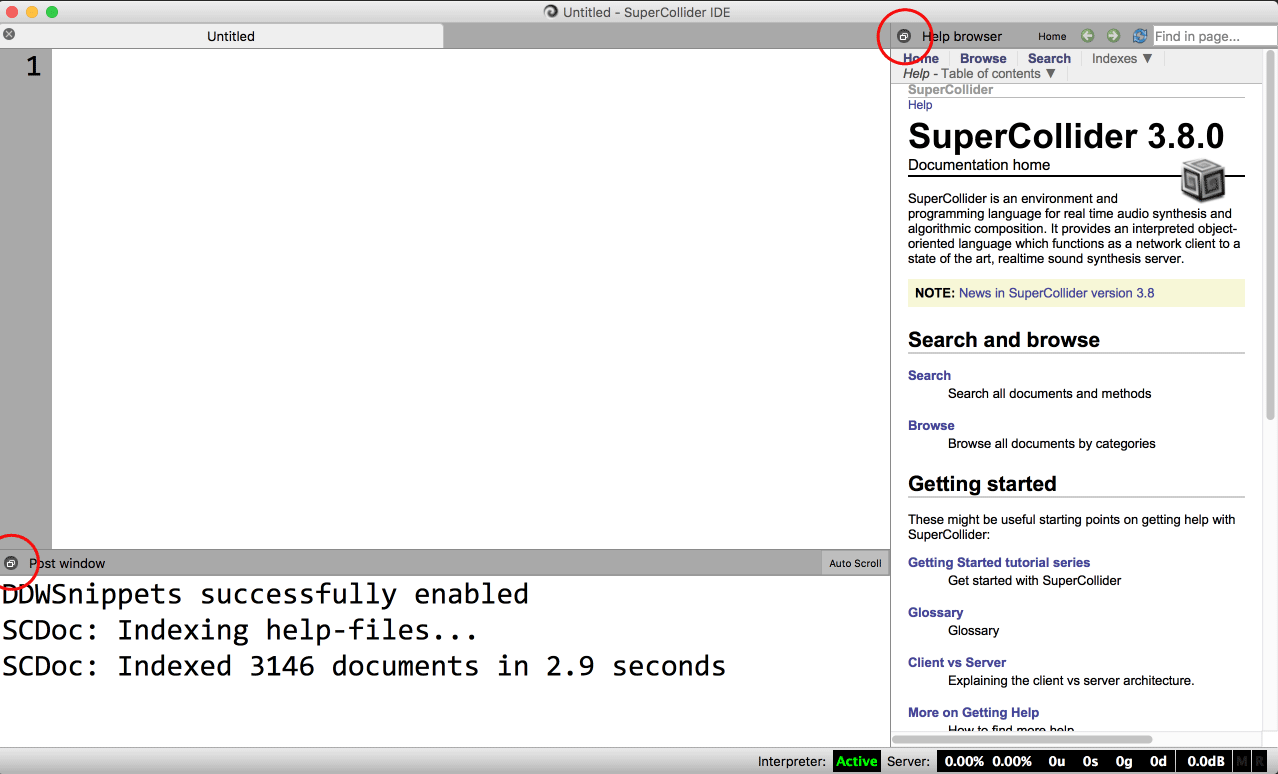
\includegraphics[scale=0.18]{interface2}
\centering
\caption{Orden de elementos}
\label{fig:orden}
\end{figure} 

\begin{itemize}
	\item Undock/Dock: monta y desmonta la ventana. Podemos arrastrarla y situarla en el sitio desado.
	\item Detach/Attach: crea una ventana flotante independiente.
	\item Close: cierra la ventana.
	\label{fig:docklets}
\end{itemize}

Si cerramos una de estas ventanas por accidente, podemos recuperarla yendo a la pestaña view/docklets:

\begin{figure}[h]
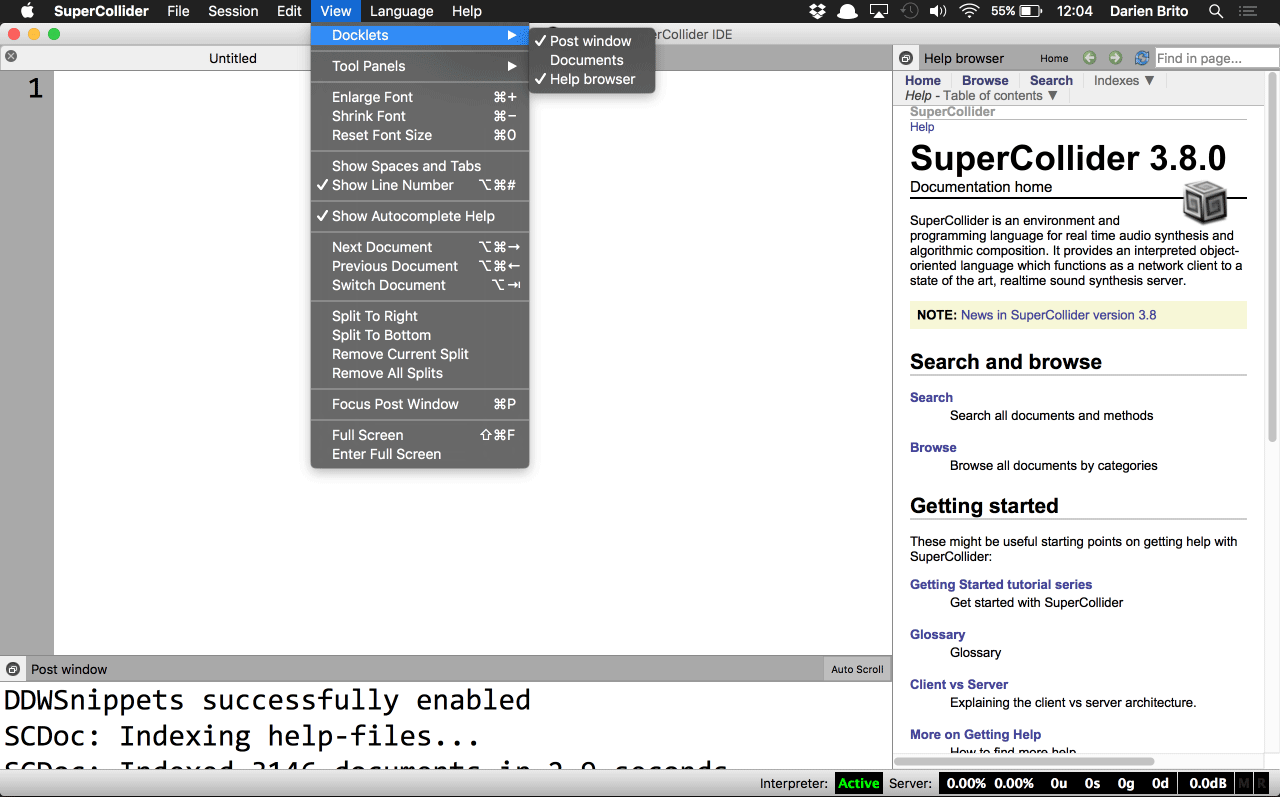
\includegraphics[scale=0.18]{interface3}
\centering
\caption{Activar docklets}
\label{fig:activar}
\end{figure} 

``Post window'' es nuestra consola y ``Help browser'' nuestra ventana de ayuda. ``Documents'' es un menú adicional que nos permite ver el directorio actual del documento en el que estamos trabajando.

Si queremos alterar los colores de la interface, podemos ir a: \\
SuperCollider/preferences/editor/Fonts\&Colors y escoger la configuración deseada. En el caso de este tutorial, yo he escogido el preset \textit{Black} y la fuente \textit{consolas}.

\section{Nociones preliminares}

Finalmente, aquí una guía con síntaxis y objetos que veremos en nuestro curso introductorio. Si la explicación en esta guía no tiene mucho sentido en este momento no hay problema. Esta aquí para prepararte y se complementa con las explicaciones del vídeo. 

\begin{itemize}

\item \textbf{Integer}: un número íntegro. ej: 1, 10, 100

\item \textbf{Float}: un número decimal. ej: 1.0, 10.0, 100.0

\item \textbf{String}: una cadena de caracteres, palabras, frase, oración o una secuencia ordenada de longitud arbitraria. Se crean con los símbolos para comillas `` ''. Por tanto, todo dentro de estos símbolos se convierte en una String, incluso números. ej: ``hola'', ``otra cosa'', ``123.1''.

\item \textbf{Comentarios}: texto que no es evaluado por el intéprete. Se usan para dejar notas o aclaraciones en un programa. Se crean con los símbolos: 
\begin{verbatim} 
// 
\end{verbatim}
Todo lo posterior a estos símbolos se convierte en un comentario a menos que creemos una nueva linea. A traves de nuestro tutorial, encontrarás varios comentarios que aclaran líneas de código. ej:

\begin{verbatim} 
SinOsc.ar() // este es un oscilador sinusoide
\end{verbatim}

Para comentarios multi-línea podemos usar los símbolos:

\begin{verbatim} 
/*   */ 
\end{verbatim}

Todo lo que va dentro de estos símbolos se convierte en un comentario. ej:

\begin{verbatim} 
/*
Todo esto es un comentario.

Puedo crear varias líneas.
*/
\end{verbatim}

\item \textbf{Array}: una colección de elementos. Un Array se crea con los símbolos: 
\begin{verbatim} 
[ ] 
\end{verbatim} 
Un array sirve para almacenar varios objetos en una sola caja, por así decirlo. Podemos acceder a los elementos de esta caja usando un número índice, que es la posición del objeto en el Array. ej: 
\begin{verbatim} 
[1, 10.0, ``hola''] 
\end{verbatim}

\item \textbf{Punto y coma (;)}: El punto y coma sirve para decirle al intérprete que una instrucción determinada a concluido. A través de los programas que escribamos verás como separar instrucciones usando este símbolo.

\item \textbf{var}: una variable. Se usa para referirnos a un objeto usando una palabra clave arbitraria. Esta palabra puede ser cualquier cosa siempre y cuando no inicie con mayúsculas o números y no tenga caracteres especiales como acentos. Para asignar un valor a una variable, usamos los signos de igual. ej: 

\begin{verbatim} 
var miVariable = 10;
\end{verbatim}

\item \textbf{postln}: un método. Métodos son funciones que los objetos entienden a fin de realizar una acción. El método postln se encarga de imprimir el objeto en la consola. Para usar un método, necesitamos usar antes un punto, a fin de que el intérprete sea capaz de entender en donde inicia el método. ej: 

\begin{verbatim} 
``¡Hola Mundo''.postln;
\end{verbatim}

\item \textbf{Funciones}: una función es una serie de instrucciones encapsuladas en un objeto. Se usan cuando queremos crear porciones de código re-utlizables. Se crean con los símbolos:

 \begin{verbatim} 
{ }
\end{verbatim}

Podemos asignar una función a una variable y reutilizarla a través de nuestro programa. ej:

\begin{verbatim} 
var f = { ``Hola mundo''.postln };
\end{verbatim}

Para evaluar una función usamos el método value. ej:

\begin{verbatim} 
f.value;
\end{verbatim}

\item \textbf{arg}: un argumento. Se usa para crear una compuerta a través de la cual pasar un objeto. Usamos argumentos cuando tenemos funciones que requieren valores flexibles para operar. ej: 

\begin{verbatim} 
var f = {arg i; i.postln }; // imprime el objeto en la consola
f.value(1); // imprime 1
f.value(10); // imprime 10
\end{verbatim}

\end{itemize}

\section{Usando los documentos de soporte}

Como ya hemos dicho, existen documentos de soporte en el \href{
https://github.com/DarienBrito/Quadro_SCIntro}{\textbf{repositorio}} de nuestro tutorial. La idea de estos documentos es que tengas a la mano todo lo que vamos viendo en cada vídeo. Te recomiendo realizar variaciones de cada ejercicio en los documentos por tu cuenta, a fin de entender los conceptos tal y como se van presentando. Para este propósito, he dejado un espacio entre líneas de código, de modo que te invite a experimentar un poco.

Te deseo buena suerte con este tutorial y espero que la información que encuentres te sea de ayuda. No dudes en escribir a la dirección dada en la plataforma con sugerencias o comentarios. ¡Feliz programación!

